\graphicspath{{07-Absorber/Figures/}}

\section{Liquid Hydrogen Absorber}
\label{Sect:Absorber}

The accurate characterisation of the properties of the liquid hydrogen
absorber was a critically-important contribution to the study of
ionisation cooling.
The instrumentation used for this purpose and its performance are
presented in this section.

The absorber vessel consisted of a cylindrical aluminium body sealed
with two thin aluminium end windows, as shown in
figure~\ref{Fig:AbsorberVessel:Diag}.
The absorber vessel contained 22\,l of liquid.
The body of the absorber had an inner diameter of 300\,mm and the end
flanges were separated by a distance of 230\,mm.
The vessel was surrounded by a second pair of safety
windows.
The length along the central axis, between the
two domes of the end windows, was 350\,mm~\cite{1748-0221-13-09-T09008}.
\begin{figure}
  \begin{center}
    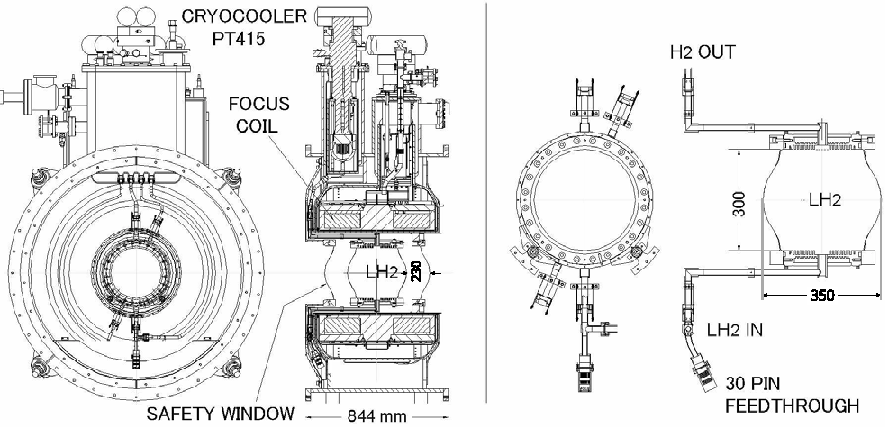
\includegraphics[width=0.80\textwidth]{AFC-drwng-edited.pdf}
  \end{center}
  \caption{
    Left panel: Drawing of the focus coil (FC) module
    showing the principal components.
    Right panel: detail of the liquid hydrogen absorber vessel~\cite{1748-0221-13-09-T09008}.
  }
  \label{Fig:AbsorberVessel:Diag}
\end{figure} \\

\noindent\textbf{Variation of the density of liquid hydrogen due to
    varying temperature and pressure} \\
\noindent
The energy lost by a muon travelling through the liquid hydrogen
absorber depends on the path length and on
the density of the liquid hydrogen. The density of liquid hydrogen is
a function of temperature and pressure.  
The temperature of the vessel was measured by eight LakeShore Cernox
1050 SD sensors, but with the values truncated for storage
at a granularity of 0.1\,K.
Four of the sensors were used solely as temperature sensors, while the
other four were also used as level sensors to ensure the
liquid hydrogen reached the top of the vessel. 
The sensors were arranged in pairs, with two mechanically clamped at
the top of the vessel, two at a polar angle of ${45}^{\circ}$ to
vertical from the top of the vessel, two at a polar angle of
${45}^{\circ}$ to the bottom of the vessel, and a
final two at at the bottom of the vessel. 

Cooldown and liquefaction were completed slowly over eight days at a
pressure of 1105\,mbar after which the vessel's pressure was lowered to
1085\,mbar~\cite{1748-0221-13-09-T09008}.
The vessel then remained in this steady state during the 21 day period of data taking, after which the vessel was vented. For the venting process,
the cryocooler used to liquefy hydrogen was
switched off and heaters were switched on to deliver a nominal power
of 50\,W to the absorber vessel.
This resulted in an increase in pressure to 1505\,mbar until the
temperature stabilised at the boiling point.
A rapid increase in temperature was observed once all the
liquid hydrogen had boiled off. 

The temperature sensors had a typical accuracy of
$\mathrm{\pm}$\,9\,mK and a long-term stability of
$\mathrm{\pm}$\,12\,mK at 20\,K.
The magnetic-field dependent temperature error, $\Delta$\textit{T}/\textit{T}, at 2.5\,T is 0.04\%,
equivalent to $\mathrm{\pm}$\,8\,mK at
20\,K~\cite{TemperatureMeasurement}.
These uncertainties were quoted by the manufacturer of the sensors.
Magnetic fields caused reversible calibration shifts on the temperature
measurements.
To reduce the uncertainty in the liquid hydrogen density a calibration
procedure was devised that used the boiling point, as observed
during the venting process.
A correction to the observed temperature reading was obtained by
applying a cut-off correction, a correction for the effect of the
magnetic field based on the current in the focus coil and its
polarity, a correction for the non-linearity of the sensors, and a 
boiling point scaling factor~\cite{NOTE524}.  
 
The boiling point of hydrogen at 1085\,mbar is 20.511\,K.
The sensors had a total uncertainty of 17\,mK (9\,mK accuracy, 12\,mK
stability, 8\,mK magnetic).
The deviation from the non-linearity of the sensors~\cite{TemperatureMeasurement} added, on average,
0.03\,K to the uncertainty.
The temperature scaling and magnet-current correction factors also
had an associated uncertainty as
they were derived based on the 0.1\,K resolution of the retrieved, truncated, values.
For example, a calibrated sensor at boiling temperature and 1505\,mbar
should read 21.692\,K, but we can only retrieve a value of
21.65\,K (21.6\,K truncated plus 0.05 K cut-off correction~\cite{NOTE524}) i.e.
off by 0.042\,K.
The pressure sensors had an uncertainty of $\mathrm{\pm}$\,5\,mbar
which equated to $\mathrm{\pm}$\,0.016\,K during steady state.
The pressure uncertainty ($\mathrm{\pm}$\,5\,mbar) added another
uncertainty to the temperature calibration constants of
$\mathrm{\pm}$\,0.014\,K.
Collectively, all these uncertainties summed in quadrature to 0.2\,K for
each sensor.
 
While in the steady state condition the liquid hydrogen was close to the
boiling temperature of liquid parahydrogen~\cite{NOTE524} (density of 70.53\,kg/m$^{3}$):
the average temperature of the eight sensors was (20.51\,$\mathrm{\pm}$\,0.07)\,K at 1085\,mbar
(figure~\ref{Fig:TempCalibrated}) allowing us to determine the
uncertainty in the density over this period as 0.08\,kg/m$^{3}$. \\
\begin{figure}
  \begin{center}
    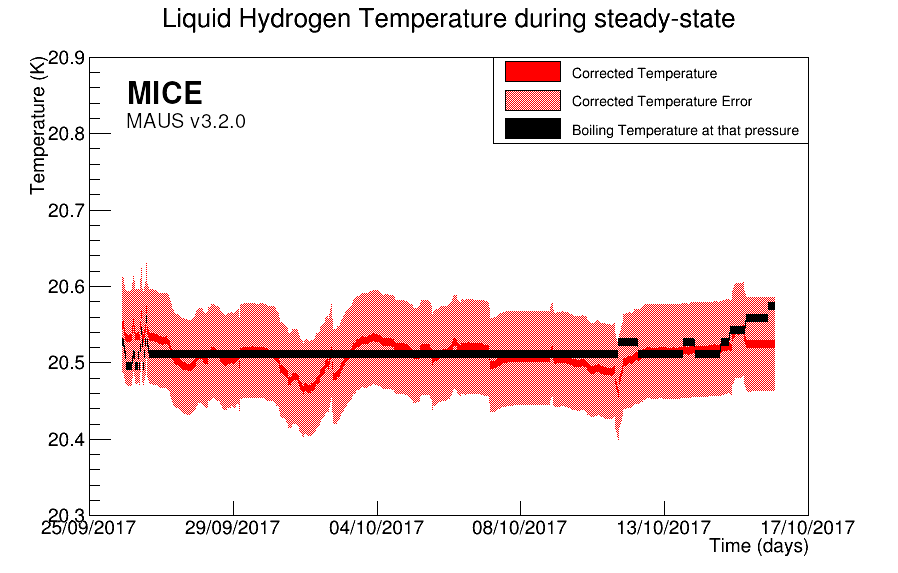
\includegraphics[width=0.80\textwidth]{SteadyState60mK_logo.png}
  \end{center}
  \caption{
    Average liquid hydrogen temperature recorded by the sensors during the
    steady state period.
    After applying all the correction factors the temperature remains
    at or close to the boiling point temperature.
  }
  \label{Fig:TempCalibrated}
\end{figure}

\noindent\textbf{Contraction of the absorber vessel due to cooling} \\
\noindent
The absorber was cooled from room temperature to the operating
temperature of the experiment (20.51\,K), contracting the vessel.
The linear contraction of Al-6061 as it is cooled from 293\,K is given
by: 
\begin{equation}
  \alpha =-4.1277\times {10}^{-3}T-3.0389\times {10}^{-6}T^2+8.7696\times {10}^{-8}T^3-9.9821\times {10}^{-11}T^4
\end{equation}
where $T$ is the operating temperature~\cite{Hardin}.
The equation is the result of a fit to data collated by the National
Institute of Standards and Technology (NIST) and has an associated
curve fit error of 4\%. 
At the MICE operating temperature, this corresponds to a linear
contraction of the vessel along each plane of 0.415\%.
As a result the length of the bore contracted by
$(1.45 \pm 0.05)$\,mm.
The vessel was suspended within the warm bore of the focus coil and
was therefore free to contract in each plane without restriction.  \\

\noindent\textbf{Deflection of absorber vessel windows due to internal
  pressure} \\
\noindent
To minimise energy loss and Coulomb scattering by the absorber vessel,
the window thickness was minimised.
The liquid hydrogen circuit was pressurised
above atmospheric pressure to prevent air ingress~\cite{1748-0221-13-09-T09008,Ishimoto}. 
The vessel was designed to withstand at least 2500\,mbar internally.
The internal pressure was limited by the 1.5\,bar relief valve to atmosphere, whilst the vessel was surrounded by vacuum.

The pressure at which the absorber operated resulted in deflection of the absorber windows. These
deflections were modelled using ANSYS~\cite{NOTE155}, and the uncertainty in the
window deflection derived from this model was 20\%.
The model showed a linear dependence of the window deflection on
pressure up to 2\,Bar when the windows begin to yield.
The pressure sensors were accurate to $\mathrm{\pm}$\,5\,mbar
(0.25\% of 2\,Bar).
At (1085\,$\mathrm{\pm}$\,5)\,mbar, the typical MICE operating
pressure, this corresponded to a deflection of
(0.5374\,$\mathrm{\pm}$\,0.1076)\,mm (model uncertainty)
$\mathrm{\pm}$\,0.0022\,mm (sensor uncertainty) at the centre of the
absorber window. \\

\noindent\textbf{Variation of the absorber vessel window thicknesses} \\
\noindent
On its passage through the absorber a muon would lose energy in the
aluminium of the pair of hydrogen-containment windows, the two
aluminium safety windows, and the liquid hydrogen itself.
At the centre of the absorber, the total amount of aluminium the muon
beam passed through was (785\,$\mathrm{\pm}$\,13)\,$\mu$m, producing a variance
of 1.68\%.
However, as the windows were thin, the effects on energy loss were
negligible.
A 200\,MeV/$c$ muon passing along the central axis of an empty
absorber lost 0.345\,MeV, introducing a 0.006\,MeV uncertainty
on energy loss.  \\

\noindent\textbf{Total systematic uncertainty on energy loss} \\
\noindent
The principal contributions to the systematic uncertainty on energy
loss in the liquid hydrogen absorber are: the uncertainty in the
contraction of the absorber vessel, the uncertainty in the deflection
of the hydrogen-containment windows due to internal pressure, and the
uncertainty in the variation of the window thickness.
The impact of the contraction of vessel and the deflection of the
windows resulted in a reduction of the length of the vessel on
axis of (0.4\,$\mathrm{\pm}$\,0.2)\,mm.
The change in the combined thicknesses of the absorber
windows on axis is 13\,$\mu$m.
The average temperature during the steady state period of the
experiment when the pressure remained constant at
(1085\,$\mathrm{\pm}$\,5)\,mbar is (20.51\,$\mathrm{\pm}$\,0.07)\,K 
corresponding to a liquid hydrogen density of (70.53\,$\mathrm{\pm}$\,0.08)\,kg/m$^{3}$.

During the MICE data taking, muon beams with nominal momenta of 140,
170, 200 and 240\,MeV/$c$ were used.
The energy loss and its uncertainty were calculated.
The calculation used a central bore length of
(349.6\,$\mathrm{\pm}$\,0.2)\,mm, a total window thickness of
(0.785\,$\mathrm{\pm}$\,0.013)\,mm and a liquid hydrogen density of
\linebreak[4] 
(70.53\,$\mathrm{\pm}$\,0.08)\,kg/m$^{3}$.
For a 140\,MeV/$c$ muon this corresponds to an energy loss of
(10.88\,$\mathrm{\pm}$\,0.02)\,MeV, while for a 200\,MeV/$c$ muon 
particle this corresponds to an energy loss of
(10.44\,$\mathrm{\pm}$\,0.02)\,MeV.
For a muon travelling along the centre axis of the absorber the
systematic uncertainty in the energy loss is 0.2\%.
